\section{TOKIO Architecture \& Implementation} \label{sec:architecture}

\begin{figure}
    \centering
    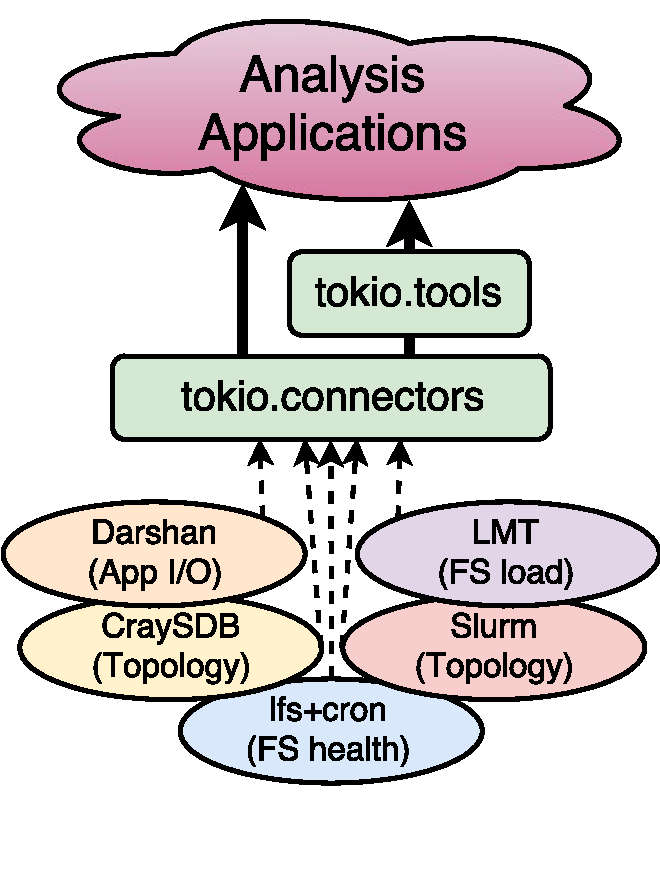
\includegraphics[width=0.7\columnwidth]{tokio-architecture-v3}
    \vspace{-.3in}
    \caption{TOKIO Architecture.  \texttt{tokio.connectors} take input from component-level monitoring tools in their native output formats and expose that data to upstream analysis in standard data formats such as key-value pairs, pandas DataFrames, and NumPy arrays. \texttt{tokio.tools} provide indices, site-specific data placement information, and enhanced usability.}
    \label{fig:tokio-architecture}
    \vspace{-.2in}
\end{figure}

To meet the design criteria outlined in Section \ref{sec:intro}, the TOKIO framework is comprised of four layers as shown in Figure \ref{fig:tokio-architecture}.
Each layer is then composed of modules which are largely independent of each other to allow TOKIO to integrate with whatever selection of tools a given HPC center has running in production.
That said, certain tools are \emph{de facto} standards for I/O performance analysis, and those tools will be highlighted in the following architectural description as examples of how TOKIO enables holistic analysis.

\subsection{Component-level monitoring tools} \label{sec:architecture/components}

Following design criterion \#\ref{design:existingtools}, TOKIO builds upon whatever monitoring and profiling tools are already in production at an HPC facility.
Although the tools and infrastructure supporting them exist outside of the scope of TOKIO, we identify several broad categories of metrics that are relevant to understanding I/O performance.

\subsubsection{Application behavior} \label{sec:architecture/components/application}

The I/O patterns that a program issues can affect performance dramatically regardless of the underlying storage system.
This behavior can be automatically profiled using tools like Darshan~\cite{Carns2009}, which is a link-time library that transparently records concise, bounded statistics about an application's I/O behavior.  
It is commonly included with all compiled applications at CUG member sites including NERSC, ALCF, NCSA, and KAUST~\cite{Lockwood2017,Luu:2015:HPDC,Hadri2015,White2017}.
Complementary information from client-side monitoring  such as the collection of file system client metric collection enabled by RUR~\cite{Butler2014} also falls in this category.

In all cases, though, understanding application behavior can yield insights into client-side caching and intra-node or intra-application contention~\cite{Lofstead2010} that may not be quantifiable from other parts of the I/O subsystem.
However, the sensitivity of application performance to jitter caused by continguous performance monitoring on compute nodes results in these application behavior data being scalar in nature; collecting these data over time can be prohibitively disruptive.

\subsubsection{Storage system traffic} \label{sec:architecture/components/fs}

The servers that serve and store file data and metadata are inherently shared by all users of an HPC system, and as a result, are intuitively susceptible to resource contention from competing jobs.
It follows that monitoring the traffic and load on each storage system server is valuable for identifying contention-related issues that may be beyond the visibility of individual users and their jobs.

Just as there are a variety of storage system implementations, there are a variety of implementation-specific tools for collecting these data.
On Cray ClusterStor systems, Lustre Monitoring Tools (LMT) have historically collected this data~\cite{Keopp2014}, and Cray's newer Caribou and Seastream infrastructure is being positioned as the preferred alternative for the future~\cite{Flaskerud2017}.
File system-specific tools for Cray DataWarp systems do not yet exist, but NERSC has demonstrated that collectd and Elasticsearch can collect and store device-level load data to similar ends~\cite{Whitney2016}.
Unlike application behavior data, collecting storage system traffic at high frequency results in minimal perceptible jitter relative to the latency of typical I/O operations.
As a result, storage system traffic is commonly recorded as time series data with an ideal sampling rate greater than ${{^1 / _{60} \textup{ Hz}}}$~\cite{Madireddy2017}.

\subsubsection{Storage system health}  \label{sec:architecture/components/fshealth}

There are many circumstances in which a component of a storage system is known to be in an available but degraded state of performance as a result of a temporary failure or condition.
Conditions such as storage device failovers (where a server may have to take on the load of a failed partner server) or RAID rebuilds (where device bandwidth is being consumed by reconstruction of data from parity) can introduce significant, long-tail performance losses to files that are striped across those degraded devices~\cite{Byna2013}.

As with storage system traffic data, storage system health data is often monitored using implementation-specific tools that understand architecture-specific failures that degrade performance.
In the case of Lustre, the \texttt{lctl dl -t} command is sufficient to identify failed-over OSTs from any Lustre client, while \texttt{lfs df} provides information that implicates performance loss due to high file system fullness.
Similarly, DataWarp can be monitored on a per-device basis using standard tools such as \texttt{smartctl} or vendor-specific tools such as the Intel SSD Data Center Tool (ISDCT)~\cite{isdct}.

\subsubsection{Job topology} \label{sec:architecture/components/topology}

The effects of locality on I/O performance within high-diameter networks have been well documented~\cite{Vishwanath2011,Bui2014,Dillow2011}, and modern high-radix topologies continue to be susceptible to topology-induced performance variation~\cite{Mubarak2017}.
Obtaining the topological mapping of a given job's compute nodes across a given network fabric requires several different tools that combine job$\leftrightarrow$node mappings from the system resource manager with the node$\leftrightarrow$coordinate mapping from the system component which tracks global system state.

In practice, both of these tool sets are highly system-specific; the job$\leftrightarrow$node mappings may be provided by a resource manager such as Slurm~\cite{Jacobsen2016} or ALPS~\cite{Karo2006}, and node$\leftrightarrow$topology mappings are provided by the Cray Service Database.
Fortunately, the relationship between nodes and topological coordinates in the fabric is a relatively static mapping, and it can be aggressively cached so long as that cache is expired any time the fabric topology is altered.

\subsubsection{Network traffic} \label{sec:architecture/components/network}

The networks over which I/O transits, including both the high-speed network and the back-end storage network, are shared resources and therefore susceptible to contention from other workloads.
Unlike the storage system traffic data, though, network traffic loads tend to be very complex since they are a function of loads at both compute and storage server endpoints as well as incidental traffic being routed over the same links.

On Cray systems, the Gemini Counter Performance Daemon~\cite{Pedretti2013,Brandt2016} or AriesNCL~\cite{ariesncl} can be used to collect the performance counters available on Aries routers.
In practice, the complexity and scale of these network traffic data make them challenging to collect effectively.
LDMS~\cite{Agelastos2014ldms} has emerged as a scalable infrastructure for collecting these data system-wide, while PAPI has been demonstrated to collect these data on a per-job basis~\cite{Groves2017}.


\begin{table*}
\centering
\setlength{\extrarowheight}{0pt}
% \addtolength{\extrarowheight}{\aboverulesep}
\addtolength{\extrarowheight}{\belowrulesep}
\setlength{\aboverulesep}{0pt}
\setlength{\belowrulesep}{0pt}
\caption{TOKIO connectors available in pytokio 0.9} \label{tab:connectors}
\begin{tabular}{llll} 
\toprule
\textbf{Connector} & \textbf{Parent Class} & \textbf{Component-Level Tool} & \textbf{Data Provided}               \\ 
\hline
CraySdb     & dict                   & Cray Service Database              & Node network topology                 \\ 
Darshan     & dict                   & Darshan 3.0 or newer               & Application-level I/O profiles        \\ 
LfsOstMap   & dict                   & Lustre \texttt{lctl dl -t}         & Failover status of OSTs and OSSes     \\ 
LfsOstFullness & dict                & Lustre \texttt{lfs df}             & Fullness of OSTs                      \\ 
LmtDb       & N/A                    & MySQL with LMT schema              & Lustre server-side traffic            \\ 
Slurm       & dict                   & Slurm                              & Job IDs, node lists, start/end times  \\ 
Hdf5        & h5py.File              & Multiple TOKIO services            & File system server-side time series   \\ 
\hdashline
CollectdEs  & N/A                    & Elasticsearch with collectd schema & Burst buffer server-side traffic      \\ 
NerscIsdct  & dict                   & ISDCT w/ NERSC directory structure & Burst buffer SSD SMART data           \\ 
NerscJobsDb & N/A                    & MySQL with NERSC accounting schema & System-wide job workload              \\
\bottomrule
\end{tabular}
\end{table*}

\subsection{TOKIO connectors} \label{sec:architecture/connectors}

The foundational layer of TOKIO are \emph{connectors}, which are independent, modular components that provide an interface between the individual component-level tools described above and the higher-level TOKIO layers described later.
Each connector interacts with the native interface of a component-level tool and provides data from that tool in the form of a tool-independent interface.

As a concrete example, consider the \emph{LMT component-level tool} which exposes Lustre file system workload data through a MySQL database hosted on the ClusterStor management node~\cite{Keopp2014}.
The \emph{LMT database connector} is responsible for establishing and destroying connections to this MySQL database as well as tracking stateful entities such as database cursors.
It also encodes the schema of the LMT database tables, effectively abstracting the specific workings of the LMT database from the information that the LMT tool provides.
In this sense, a user of the LMT database connector can use a more semantically meaningful interface (e.g., \texttt{lmtdb.get\_mds\_data()} to retrieve metadata server loads) without having to craft SQL queries or write any boilerplate MySQL code.

At the same time, the LMT database connector does \emph{not} modify the data retrieved from the LMT MySQL database before returning it.
As such, using the LMT database connector still requires an understanding of the underlying LMT tool and the significance of the data it returns.
This design decision restricts the role of connectors to being convenient interfaces into existing tools that eliminate the need to write glue code between component-level tools and higher-level analysis functions.

All connectors also provide serialization and deserialization methods for the tools to which they connect.
This allows the data from a component-level tool to be stored for offline analysis, shared among collaborators, or locally cached for rapid subsequent accesses.
Continuing with the LMT connector example, the data retrieved from the LMT MySQL database may be serialized to formats such as SQLite.
Conversely, the LMT connector is also able to load LMT data from these alternative formats for use via the same downstream connector interface (e.g., \texttt{lmtdb.get\_mds\_data()}).
This dramatically simplifies some tasks such as publishing analysis data that originated from a restricted-access data source or testing new analysis code.

The pytokio implementation of TOKIO implements each connector as a Python class.
Connectors which rely on stateful connections, such as those which load data from databases, generally wrap a variety of database interfaces.
Connectors which operate statelessly, such as those that load and parse discrete log files, are generally derived from Python dictionaries and self-populate when initialized.
Where appropriate, these connectors also have methods to return different representations of themselves; for example, many connectors provide a \texttt{to\_dataframe()} method that returns the requested connector data as a pandas DataFrame.

The initial release of pytokio, version 0.9, includes the connectors listed in Table \ref{tab:connectors}.
The first six connectors listed (CraySdb through Slurm) connect to component-level tools that are either pre-installed on Cray XC and ClusterStor systems or commonly deployed open-source tools.
The latter three connectors (\mbox{CollectdEs}, \mbox{NerscIsdct}, and \mbox{NerscJobsDb}) rely on third-party infrastructure and/or use non-default schemata or encoding to represent data.
That said, these three connectors contain the logic necessary to create more generic connectors for consuming output from sources like Elasticsearch (from \mbox{CollectdEs}) or \mbox{smartctl} (from \mbox{NerscIsdct}).
Finally, the Hdf5 connector provides an interface into the TOKIO Time Series data format, a derivative of HDF5 that is used to store file system traffic data in a connector-agnostic format.
This TOKIO Time Series format is described in more detail in Section \ref{sec:apps/services}.

\subsection{TOKIO tools} \label{sec:architecture/tools}

\begin{figure}
    \centering
    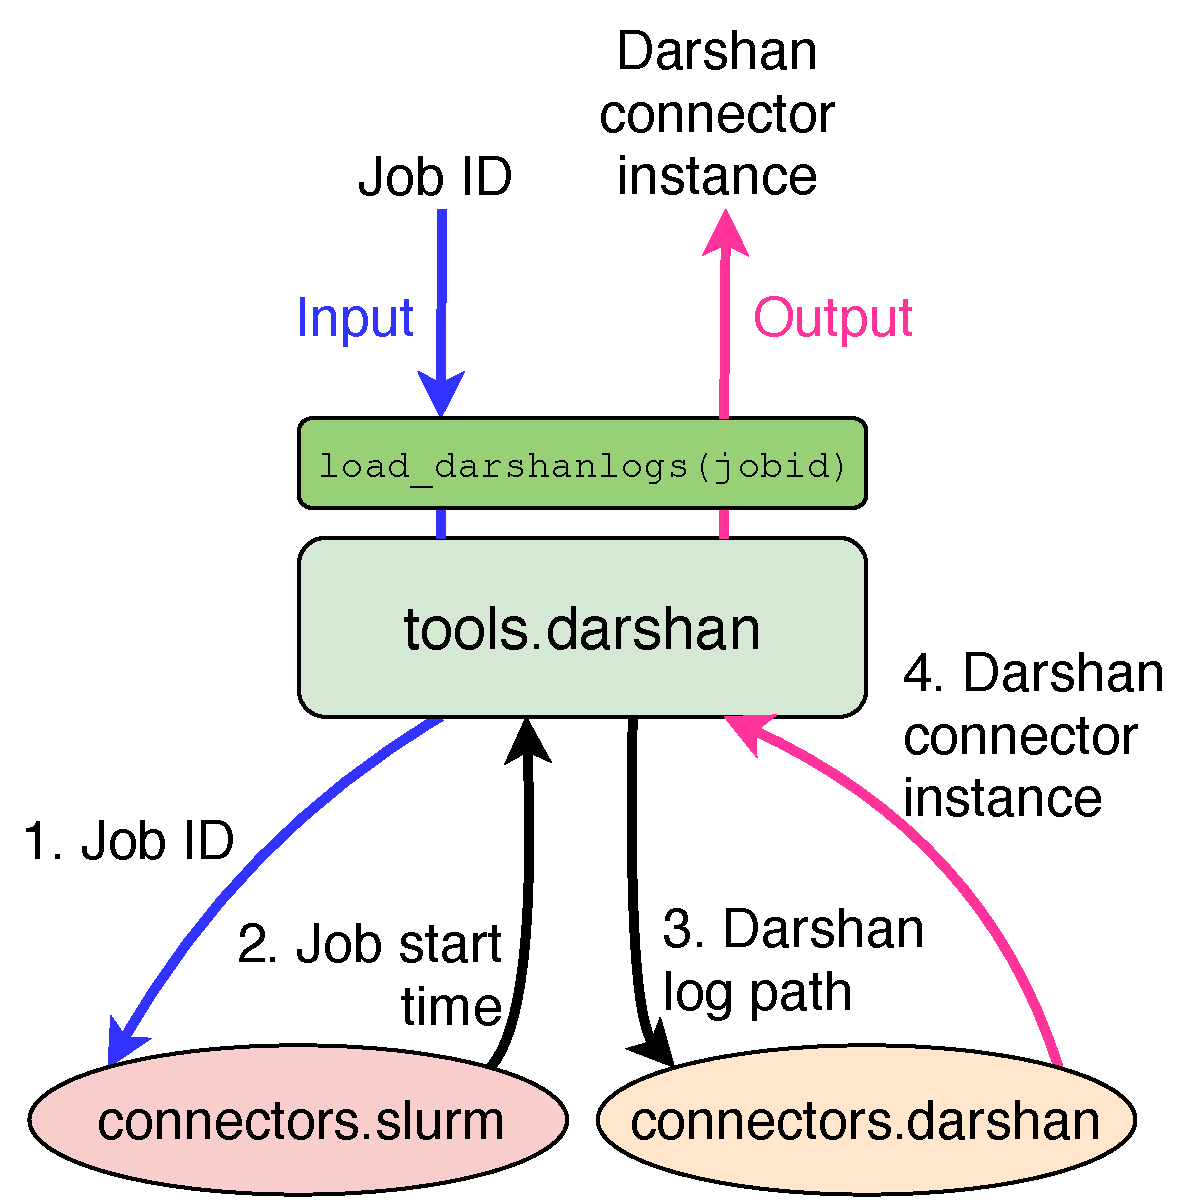
\includegraphics[width=0.7\columnwidth]{darshan-tool}
    %\vspace{-.3in}
    \caption{Darshan tools interface for converting a Slurm Job ID into Python interfaces into one or more Darshan logs.
    User specifies a Slurm Job ID; the Darshan tool retrieves the date this job ran from Slurm, and then uses this date to find the location of any relevant Darshan logs in the site-wide Darshan log repository.
    The tool then connects to each log and returns a dictionary-like Darshan connector instance for each.}
    \label{fig:darshan-tool}
    \vspace{-.2in}
\end{figure}

TOKIO \emph{tools} are implemented on top of connectors as an optional set of interfaces that are semantically closer to how analysis applications may wish to access component-level data.
To this end, the TOKIO tools interfaces typically serve two purposes:
encapsulating site-specific information on how certain data sources are indexed or where they may be found, and
providing higher-level abstractions atop one or more connectors to mask the complexities or nuances of the underlying data sources.

\subsubsection{Encapsulating site-specific information}

pytokio factors out all of its site-specific knowledge from connectors into a single site-specific configuration file.
This configuration file is composed of arbitrary JSON-encoded key-value pairs which are loaded whenever pytokio is imported, and the specific meaning of any given key is defined by whichever tool accesses it.
Thus, this site-specific configuration data does not prescribe any specific schema or semantic on site-specific information, and it does not contain any implicit assumptions about which connectors or tools are available on a given system.

To illustrate this more concretely, consider the case of the Darshan component-level tool~\cite{Carns2009}.
When deployed system-wide, Darshan automatically saves users' output logs to a pre-defined, site-wide log repository.
This repository is structured such that logs are indexed by year, month, and day, and Darshan encodes a variety of metadata (including the user name, executable name, and job id) in each log file's file name.
The Darshan \emph{tool} contains the logic required to find Darshan log files in this site-wide repository when given any or all of these metadata attributes.
The top-level directory of the site-wide Darshan log repository (e.g., \texttt{{/global/darshanlogs/}}) is site-specific and therefore stored in the pytokio configuration file.
However, the directory structure \emph{within} that log repository is dictated by Darshan itself, so the mapping between dates and subdirectories is implemented within the Darshan tool.
It is then the responsibility of the Darshan connector to provide an interface into an individual Darshan log file.

\subsubsection{Providing higher-level abstractions atop connectors}

The other role of TOKIO tools are to combine site-specific knowledge and multiple connectors to provide a simpler set of interfaces that are semantically closer to a question that an I/O user or administrator may actually ask.
Continuing with the Darshan tool example from the previous section, such a question may be, ``How many GB/sec did job \#2468187 achieve?''
Answering this question involves several steps:

\begin{enumerate}[leftmargin=*]
\item Retrieving the start date for job id \#2468187 from the system workload manager or a job accounting database
\item Looking in the Darshan repository for logs that match jobid=2468187 on that date
\item Running the ``\texttt{darshan-parser --perf}'' tool on the matching Darshan log and retrieve the estimated maximum I/O performance
\end{enumerate}

pytokio provides connectors and tools to accomplish each one of these tasks:

\begin{enumerate}[leftmargin=*]
\item The \textbf{Slurm connector} provides \texttt{get\_job\_startend()} which retrieves a job's start and end times when given a Slurm job id
\item The \textbf{Darshan tool} provides \texttt{find\_darshanlogs()} which returns a list of matching Darshan logs when given a job id and the date on which that job ran
\item The \textbf{Darshan connector} provides \texttt{darshan\_parser\_perf()} which retrieves I/O performance data from a single Darshan log
\end{enumerate}

Because this is such a routine process when analyzing application I/O performance, the Darshan tools interface implements this entire sequence in a single, higher-level function called \texttt{load\_darshanlogs()}.
This function, depicted in Figure \ref{fig:darshan-tool}, effectively links two connectors (Slurm and Darshan) and provides a single function to answer the question of ``how well did job \#2468187 perform?''
This greatly simplifies the process of developing user-facing tools to analyze Darshan logs.
Any analysis tool which uses application I/O performance and operates from job ids can replace hundreds of lines of boilerplate code with a single function call into the Darshan tool, and it alleviates users from having to understand the Darshan log repository directory structure to quickly find profiling data for their jobs.

\subsubsection{Simplifying portability}

TOKIO tools interfaces are also what facilitate portable, highly integrated analyses and services for I/O performance analysis.
In the aforementioned examples, the Darshan tools interface assumes that Slurm is the system workload manager and the preferred way to get start and end times for a job id.
However, there is also a more generic jobinfo tool interface which serves as a connector-agnostic interface that retrieves basic job metrics (start and end times, node lists, etc) using a site-configurable, prioritized list of connectors.

Consider the end-to-end example shown in Figure \ref{fig:portability-flow}.  
In this case, an analysis application's purpose is to answer the question, ``What was a job's I/O performance?''
To accomplish this, the analysis takes a job id as its sole input and makes a single call into the pytokio Darshan tool's \texttt{load\_darshanlogs(jobid)} function as previously described.
The Darshan tool first uses the jobinfo tool to convert the job id (1) into a start/end time in a site-independent way.
The jobinfo tool examines the site configuration and determines that the Slurm connector is the best way to convert the job id (2) into a job start/end time (3), which is passed back to the Darshan tool (4).
The Darshan tool then uses the job start time to determine where the job's Darshan log is located in the site-specific repository, and uses this log path (5) to retrieve a connector interface into the log (6).
The Darshan tool returns this connector interface to the analysis application (7), which extracts the relevant performance metric (8) and returns it to the end user.

Through this entire process, the analysis application's only interface into pytokio was a single call into the Darshan tools interface.
Beyond this, pytokio was responsible for determining both the proper mechanism to convert a job id into a job start time and the location of Darshan logs on the system.
Thus, this analysis application is entirely free of site-specific knowledge and can be run at any HPC center to obtain I/O performance telemetry when given a job id.
The only requirement is that pytokio is installed at the HPC center, and it is correctly configured to reflect that center's site-specific configurations.

\begin{figure}
    \centering
    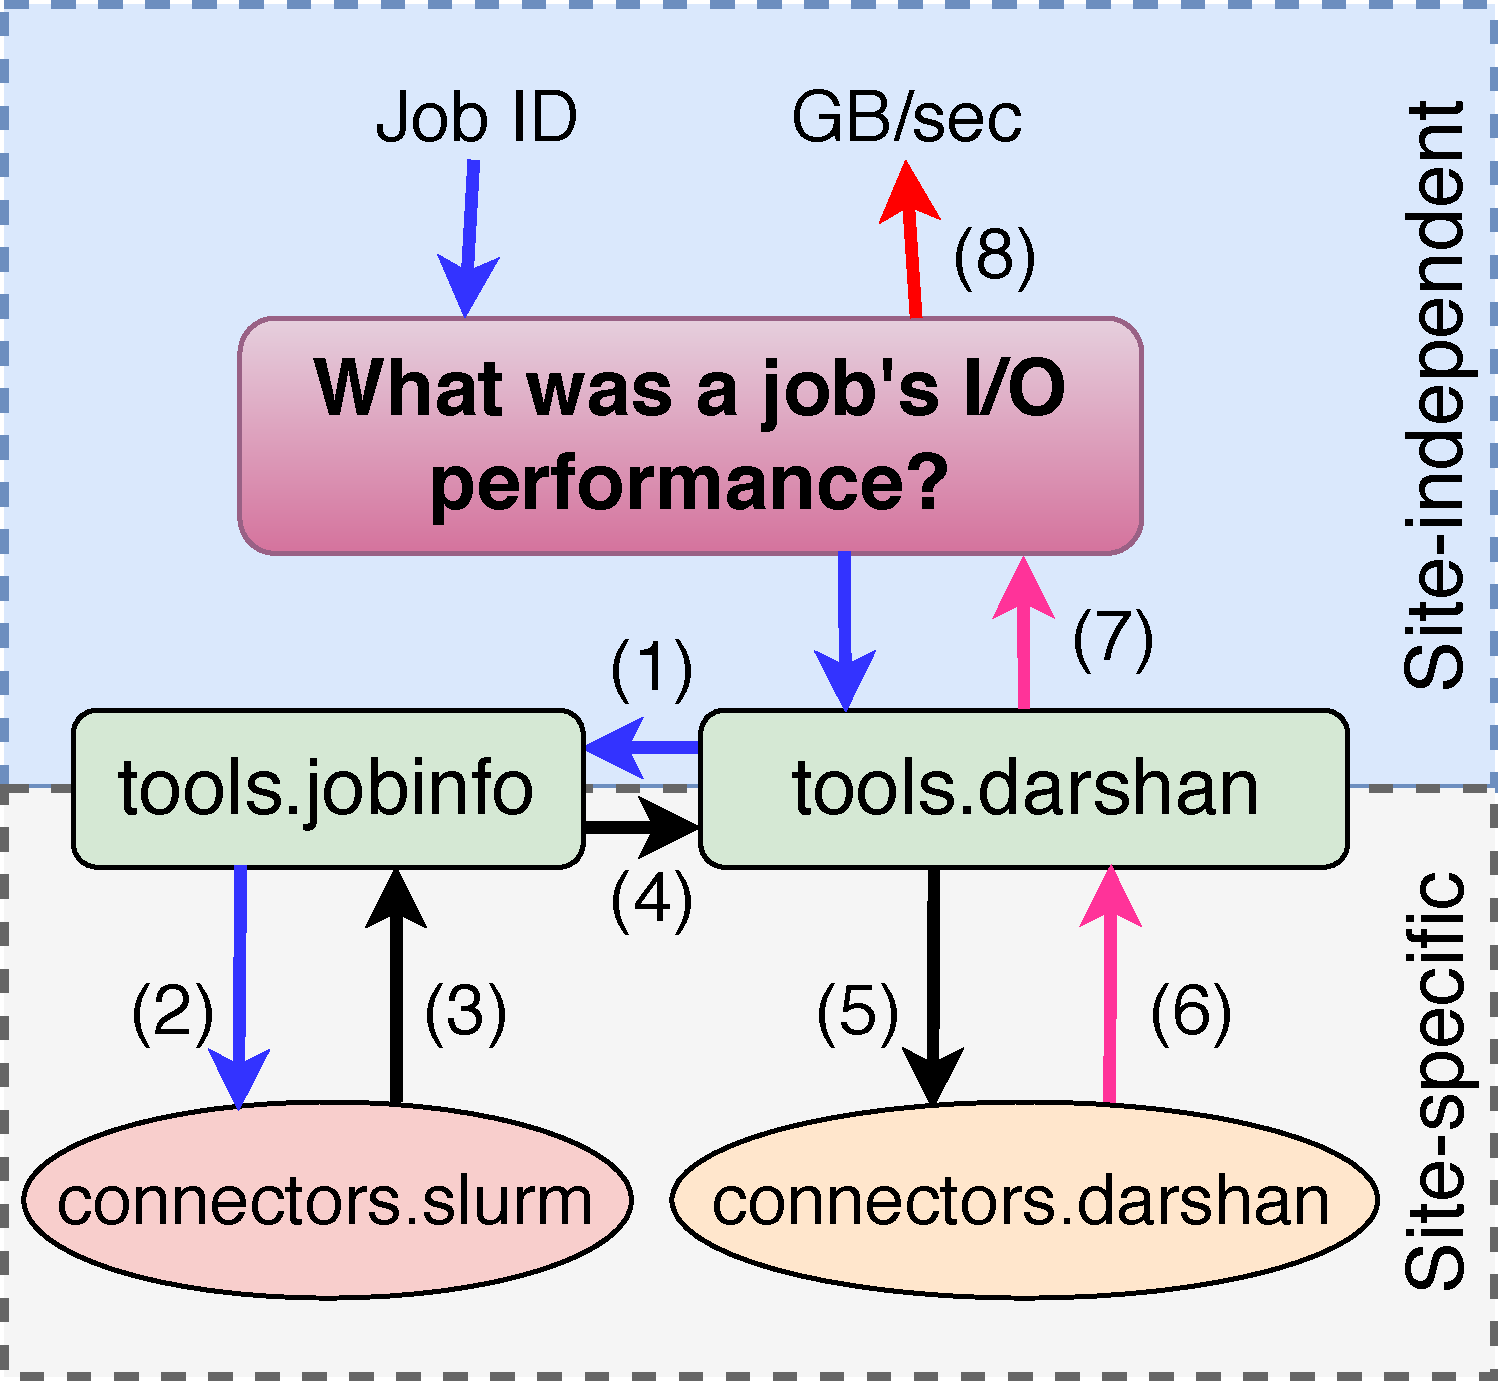
\includegraphics[width=0.7\columnwidth]{portability-flow}
    %\vspace{-.3in}
    \caption{TOKIO tools interfaces to enable portability.
    An analysis application answers the question, "What was a job's I/O performance," and it accepts the job's ID as its sole input.
    The TOKIO tools interface abstracts all of the site-specific information (such as how job ids are mapped to job start times and where Darshan logs are saved) from the higher-level analysis application.
    Thus, the analysis application can be run at any HPC center without modification provided that center has pytokio installed and correctly configured.
    }
    \label{fig:portability-flow}
    \vspace{-.2in}
\end{figure}